\chapter{Location matching}
\label{ch_matching}

The HMM method as well as the $k$-means method offer us with the possibility of
extracting locations over a given number of days. However, both the algorithms
perform better when the given time frame is shorter. This finding has come up
while carefully observing the results for different number of days for which the
algorithms have been executed.

The reason behind this behaviour seems to be the limitation of the $10$-fold
cross validation which has been used in order to evaluate the fitness of the
results. The method implies that the data from the time frame taken into
consideration is divided into $10$ equal subsequences which are afterwards used
in turns as training data and as testing data. However, when the data size grows,
the randomly divided subsequences also grow. When we are dealing with
subsequences which have a considerable size, it can happen that some of the
subsequences can contain all of the fingerprints which can be attributed to a
certain location and as such, that location cannot be estimated based on the
other subsequences which have no knowledge of it. This leads to a decay in the
efficiency of estimating the number of locations that we can expect the user
to have been at throughout the evaluated time. The current chapter explores some
possibilities that can help solve this problem.

\section{Methods for solving the ``matching of locations'' problem}

A solution for the previously mentioned problem can be to scale the $k$ factor
of the $k$-fold validation in order to use a factor larger than $10$ when
dealing with bigger amount of data, however this leads to a very long processing
time which can be avoided by using another solution. The second solution is to
extract locations for each day and concatenate the results for all the days
afterwards. This however leads to a new situation. We need to find a way in
which to identify that a location $L_{x}$ from day X might be the same as a
location $L_{y}$ from day Y. This problem is referred to in the present paper
as the ``matching of locations'' problem.

We have taken into consideration three possible ways in which we can solve this
new problem. In order to evaluate the proposed solutions we have evaluated the
results using a graphical approach. We have employed the solutions for a
selection of users for whom we have used the HMM algorithm to identify
locations through a large number of days. Using each proposed solution we have
matched the locations throughout the days and we have observed the accuracy of
the matching that was done.

\subsection{Dictionary of locations based on APs}
\label{dictionary_aps}
The algorithm which can be used for matching up locations over time based on a
\textit{dictionary based on APs} is as follows:
\begin{itemize}
  \item For each location we reunite the time bins that have been associated
  with it. We identify the APs present in either of the time bins and we consider
  all these APs to be associated to the given location
  \item Before adding a new entry in the dictionary~\footnote{Adding an entry
  in such a dictionary is equivalent with defining a new location based on the
  APs of which presence the new location is characterized by.}, we can first
  check the dictionary for previously defined locations that seem to resemble
  the new one based on the APs that define them
  \item If we do not find a similar location we can just add a new entry for the
  new location in the dictionary
  \item If we find locations which resemble the new one in a proportion bigger
  than a given threshold (they have a sufficient number of APs that coincide
  with the ones associated to the new location), we can choose the one which
  resembles the most and consider that the new location and this specific
  location are the same
  \item In the above case, the entry for the location in the dictionary is
  updated to contain the reunion of the APs which define the previous definition
  of the location and the newly found location that matches it
\end{itemize}

This method seems to be a simple solution, however, at a close exploration of
possible situations which can appear within our data we identified a case in
which this solution fails. Let us explore the situation in
Fig.~\ref{overlap_of_aps}. 

\begin{figure}[!h]
\centering
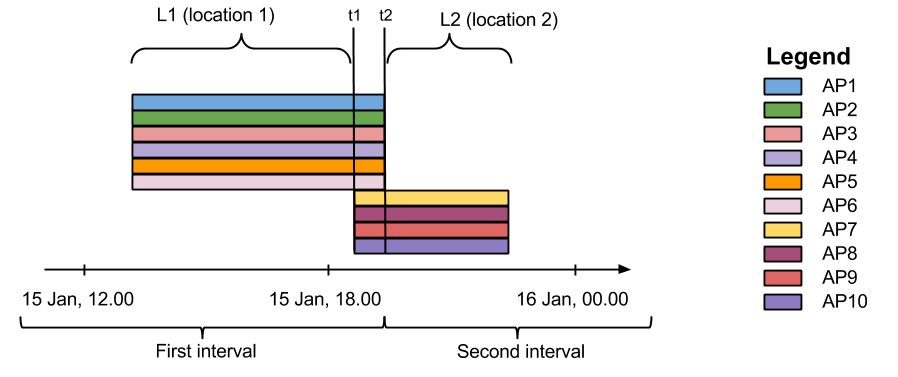
\includegraphics[width=0.95\textwidth]{figures/matching/overlap_of_aps.png}
\caption{Example of APs overlapping}
\label{overlap_of_aps}
\end{figure}

In this case the user would spend most of his or her time for the exemplified
duration at location L1 or at location L2. However, these locations can be, for
example, two rooms which are close enough so as to have a signal overlap between
them (e.g. between t1 and t2). If the user is to stop for enough time, but not
very long (e.g. $5$ minutes which is the duration of exactly one time bin) in an
intermediate location where the signals from the APs in the two rooms overlap,
then the extraction algorithm would identify the location as one of either L1 or
L2. When using the matching algorithm, the dictionary will contain an entry for
L1 which has all the APs from $1$ to $10$ as all of them have been identified
throughout the time in which the user seems to be situated at location L1.
Because of this, when the algorithm tries to see if location L2 can be matched
with another previous location, since the APs attributed to L2 are AP7-AP10,
then all of them can also be found in the entry existing for location L1 and as
such the algorithm considers that locations L1 and L2 are the same.

Situations like this one make the use of this particular algorithm to be
inefficient.

\subsection{Dictionary of locations based on fingerprints}
\label{dictionary_fingerprints}
The algorithm which can be used for matching up locations over time based on a
\textit{dictionary based on fingerprints} is as follows:
\begin{itemize}
  \item For each location identified with our location extraction algorithm and
  for each time bin in which the location appears we can see which is the
  fingerprint~\footnote{A fingerprint is calculated for each time bin. It is a
  list with $N$ elements, where $N$ is the number of APs which are associated
  with the given user. Element at position $i$ in the list is attributed to $AP_{i}$.
  Each element can be either $0$ or $1$ marking the absence or presence in the
  given time bin of the AP which corresponds to the element.} for the given time bin 
  \item An entry in the dictionary can contain the fingerprints which are
  extracted from the time bins that are associated to the location for which
  the entry is created
  \item Before adding a new entry in the dictionary, we can first
  check the dictionary to see if any previously defined location might fit the
  characteristics of the new location we are trying to add~\footnote{Meaning
  that a high number of fingerprints are common to both locations}
  \item If a similar location is not found, we can proceed with adding a new
  entry in the dictionary for the new location
  \item If we find locations which resemble the new one in a proportion bigger
  than a given threshold (which happens when they have sufficient fingerprints
  in common), we can chose the one which resembles the most and consider that
  they are the same
  \item In the above case, the entry for the location in the dictionary
  is updated to contain the reunion of the fingerprints which are attributed
  to the previously defined locations which are now matched into one
\end{itemize}

This solution eliminates the problem that was found in
Section~\ref{dictionary_aps} since, in this case the entries for location L1 and
L2 would be different as it can be seen in
Tab.~\ref{tab:table_fingerprints}~\footnote{We make the assumption that the
algorithm for extracting locations associates the period between t1 and t0 to
location L1.}.

\begin{table}[!h]
\begin{tabular}{|c|c|c|c|}
\hline
\multicolumn{1}{|l|}{}       & \multicolumn{2}{c|}{\textbf{Location 1 (L1)}}   & \textbf{Location 2 (L2)} \\ \hline
\textbf{Access points (APs)} & \textbf{Fingerprint 1} & \textbf{Fingerprint 2} & \textbf{Fingerprint 1}   \\ \hline
AP1                          & 1                      & 1                      & 0                        \\
AP2                          & 1                      & 1                      & 0                        \\
AP3                          & 1                      & 1                      & 0                        \\
AP4                          & 1                      & 1                      & 0                        \\
AP5                          & 1                      & 1                      & 0                        \\
AP6                          & 1                      & 1                      & 0                        \\
AP7                          & 0                      & 1                      & 1                        \\
AP8                          & 0                      & 1                      & 1                        \\
AP9                          & 0                      & 1                      & 1                        \\
AP10                         & 0                      & 1                      & 1                        \\ \hline
\end{tabular}
\caption{This table shows the fingerprints for locations L1 and L2 in
Fig.~\ref{overlap_of_aps}}
\label{tab:table_fingerprints}
\end{table}

There is, however, another situation which we were able to identify and which
creates difficulties for the good functionality of the present algorithm. The
mentioned case can be seen in Fig.~\ref{diff_fp_same_loc}

\begin{figure}[!h]
\centering
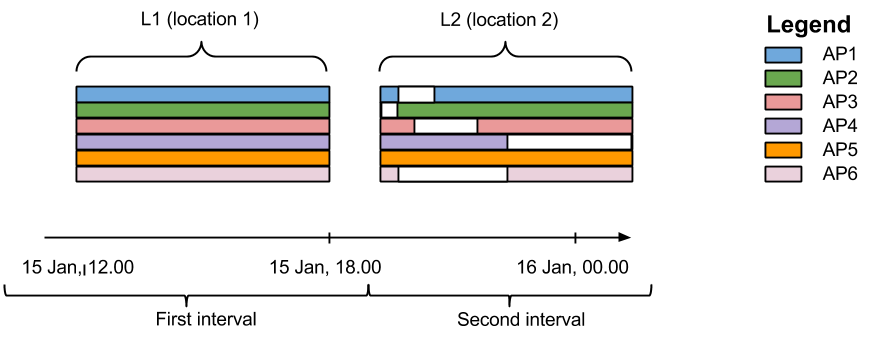
\includegraphics[width=0.95\textwidth]{figures/matching/different_fp_same_loc.png}
\caption{Example of locations which can be matched yet do not have any identical
fingerprints overlapping}
\label{diff_fp_same_loc}
\end{figure}

The fingerprints of locations L1 and L2 in this new case can be seen in
Tab.~\ref{tab:table_fingerprints_same_loc}. As we can see there are no common
fingerprints identified for the two locations because in the case of location L2
the signal from the APs that identify with it is not constant because of
possible interferences. In this case the algorithm will fail to identify the two
location as being the same one and, as such, the present algorithm can present
difficulties when solve the matching problem.

\begin{table}[!h]
\begin{tabular}{|c|c|c|c|c|c|c|c|}
\hline
             & \textbf{Location 1 (L1)}     & \multicolumn{6}{c|}{\textbf{Location 2 (L2)}}                                           \\ \hline
\textbf{APs} & \textbf{Fingerprint 1 (FP1)} & \textbf{FP1} & \textbf{FP2} & \textbf{FP3} & \textbf{FP4} & \textbf{FP5} & \textbf{FP6} \\ \hline
AP1          & 1                            & 1            & 0            & 0            & 1            & 1            & 1            \\
AP2          & 1                            & 0            & 1            & 1            & 1            & 1            & 1            \\
AP3          & 1                            & 1            & 1            & 0            & 1            & 1            & 0            \\
AP4          & 1                            & 1            & 1            & 1            & 1            & 0            & 1            \\
AP5          & 1                            & 1            & 1            & 1            & 1            & 1            & 1            \\
AP6          & 1                            & 1            & 0            & 0            & 0            & 1            & 0            \\ \hline
\end{tabular}
\caption{This table shows the fingerprints for locations L1 and L2 in
Fig.~\ref{diff_fp_same_loc}}
\label{tab:table_fingerprints_same_loc}
\end{table}

\subsection{Dictionary of location signatures}
\label{dictionary_signatures}
We define the signature of a location as follows:
\begin{itemize}
  \item It is an entity which is calculated for a location taking into
  consideration a given period of time (for example $1$ day) for which we have
  used an algorithm for extracting the locations
  \item It is an entity which identifies a location independently of the moment
  of time inside the time frame for which it is calculated (as opposed to the
  fingerprints that have been mentioned in 
  Section~\ref{dictionary_fingerprints} and which are extracted for each time bin)
  \item It is a list of $N$ elements (where $N$ is the number of APs which the
  user is associated with)
  \item Each element has the value $1$ or $0$
  \item If the element at position $i$ in the list (where $i \in \{1..N\}$) is
  $1$ it means that the associated AP ($AP_{i}$) has been found mostly with the
  value $1$ in the fingerprints associated to the existing time bins (as
  presented in Section~\ref{dictionary_fingerprints}) and if it is $0$
  it means the opposite~\footnote{This means that if the signature of the
  location we are interested in has the element attributed to a given AP set to
  $1$ then the AP has appeared in more time bins than the ones it was missing
  from during the given time frame. If it is $0$, than the AP has been missing
  from more time bins than the ones that it was present in and that are
  associated to the give location.}
\end{itemize}

The way in which these signatures are create eliminates the problems that can
appear in case interferences appear and disturb the presence of the signal from
various APs for a limited amount of time. The location matching algorithm, in
this case, can be as follows:

\begin{itemize}
  \item We calculate the location signature for each location identified with
  our location extraction algorithm throughout a given number of days
  \item An entry (which is associated to a location) in the dictionary contains
  the location signature
  \item Before adding a new entry in the dictionary, we can first
  check the dictionary to see if any of the previous locations have a signature
  that is similar above a selected threshold to the one of the new location we
  are trying to add
  \item If a similar location is not found, we can proceed with adding a new
  entry in the dictionary for the new location
  \item If we find a location which resembles the new one in a proportion bigger
  than a given threshold then we can consider that the two are the same
  location
\end{itemize}

The similarity between two signatures is calculated by taking into consideration
the APs that are set to $1$ in either of the two signatures and the APs which
are set to $0$ but that are present in both signatures~\footnote{The difference
in APs in signatures is given by the fact that, when looking at data from
different days, the APs which are scanned during these days might not always be
the same. We are not keeping all the APs associated at any moment with a user
because this leads to an unnecessary increase in the execution time.}. The
similarity value si calculated as the number of APs that have the same value
associated to them in both the signatures (either $0$ or $1$) and this number is
then divided to the number of APs in the reunion.

The similarity result obtained for two signatures is compared to a given
threshold in order to determine if the two signatures are referring to the
same geographical location. We have experimented with threshold values between
$65\%$ - $98\%$ and the results show that threshold values inside the
interval $75\%$ - $80\%$ return the most accurate results for matching
locations.

By analysing data for different users we found a case in which this method did
not identify correctly that two locations where in fact the same one. The
situation can be seen in Fig.~\ref{same_location_less_than_threshold}.

\begin{figure}[!h]
\centering
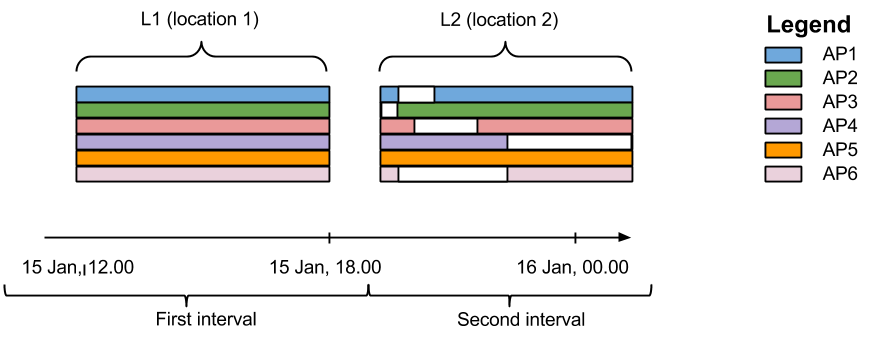
\includegraphics[width=0.95\textwidth]{figures/matching/different_fp_same_loc.png}
\caption{Example of locations which need to be matched despite their similarity
being below the threshold}
\label{same_location_less_than_threshold}
\end{figure}

As we can see, location L1 has $10$ APs while location L2 has only $5$. Since
the APs in location L2 are also present in location L1 it is safe to assume that
the remaining APs are not present in L2 due to technical problems or
interferences. However, when calculating the signatures of the two locations and
comparing them, by using a threshold value of $80\%$ for considering them the
same, we would only obtain that they are similar in a $50\%$ proportion. In
order to avoid this kind of situations, we have added to our algorithm another
condition which goes as follows: if all the APs which have the value $1$ in the
signature of a location appear in the signature of an already found previous
location, than the two can be considered the same location even if the
similarity value is not above the given threshold. This small improvement
ensures that the algorithm performs well even despite cases as this one.

This third possible solution performs well for the test we have conducted over
or data and as such it has been chosen for solving the matching problem for
locations over different days.
